\documentclass[12pt,a4paper, margin=1in]{article}
\usepackage{fullpage}
\usepackage{amsfonts, amsmath, pifont}
\usepackage{amsthm}
\usepackage{amsmath}
\usepackage{geometry}
\usepackage{graphicx}
\usepackage{float}
\graphicspath{{assets/}}

\geometry{
    a4paper,
    % total={210mm,297mm},
    left=10mm,
    right=10mm,
    top=5mm,
    bottom=10mm
}

\author{
    Ahmet Eren Çolak\\
    \texttt{e2587921@ceng.metu.edu.tr}
}

\title{ 
    \textbf{CENG 499 - Introduction to Machine Learning} \\ Homework 2
}

\renewcommand{\thesection}{\arabic{section}}

\begin{document}

\maketitle

\noindent\rule{19cm}{1.2pt}

\tableofcontents

\bigskip
\noindent\rule{19cm}{1.2pt}


\section{Part 2}

\subsection{Dataset 1}

\begin{table}[H]
    \centering
    \begin{tabular}{|c|c|c|}
    \hline
    \textbf{ID} & \textbf{C} & \textbf{Kernel} \\ \hline
    1           & 0.5        & Poly           \\ \hline
    2           & 0.5        & RBF   \\ \hline
    3           & 2          & Poly         \\ \hline
    4           & 2          & RBF   \\ \hline
    \end{tabular}
    \caption{Hyperparameter configurations}
\end{table}

I trained and tested all hyperparameters on the same training and test set. Accuracy table and decision boundaries for each hyperparameter
configuration are plotted below.

\begin{table}[H]
    \centering
    \begin{tabular}{|c|c|c|}
    \hline
    \textbf{ID} & \textbf{Accuracy} \\ \hline
    1           & 0.68              \\ \hline
    2           & 1.0               \\ \hline
    3           & 0.69              \\ \hline
    4           & 1.0               \\ \hline
    \end{tabular}
    \caption{Accuracies for each configuration}
\end{table}

\begin{figure}
    \centering
    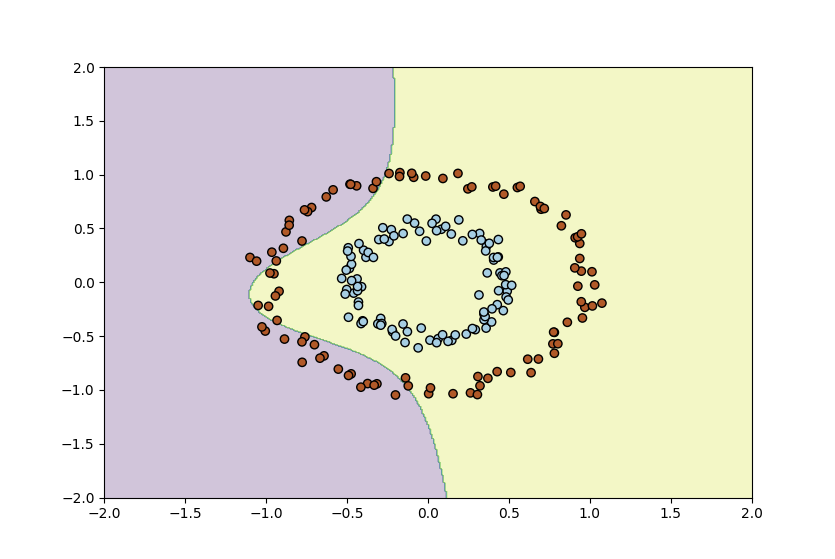
\includegraphics[scale=0.75]{svm-poly-05}
    \caption{Decision boundary of SVM with C = 0.5 and polynomial kernel}
\end{figure}
\begin{figure}
    \centering
    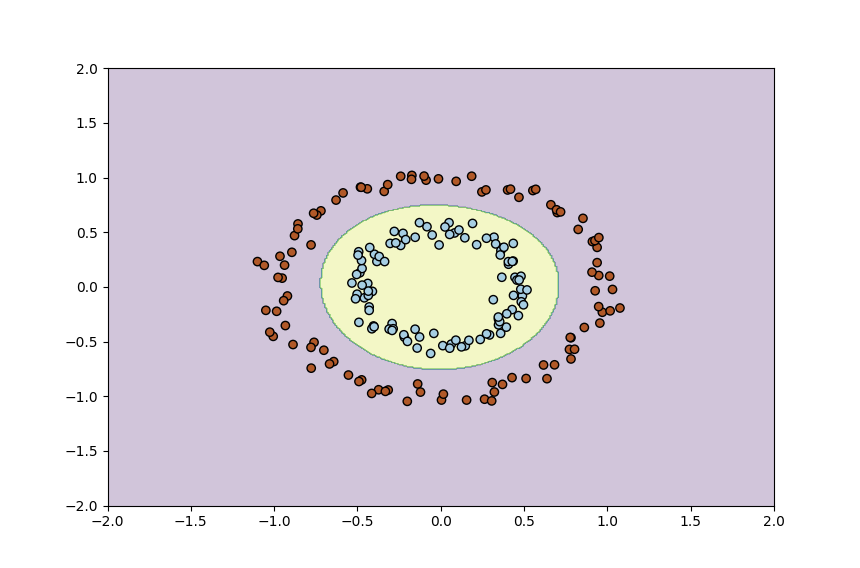
\includegraphics[scale=0.75]{svm-rbf-05}
    \caption{Decision boundary of SVM with C = 0.5 and rbf kernel}
\end{figure}
\begin{figure}
    \centering
    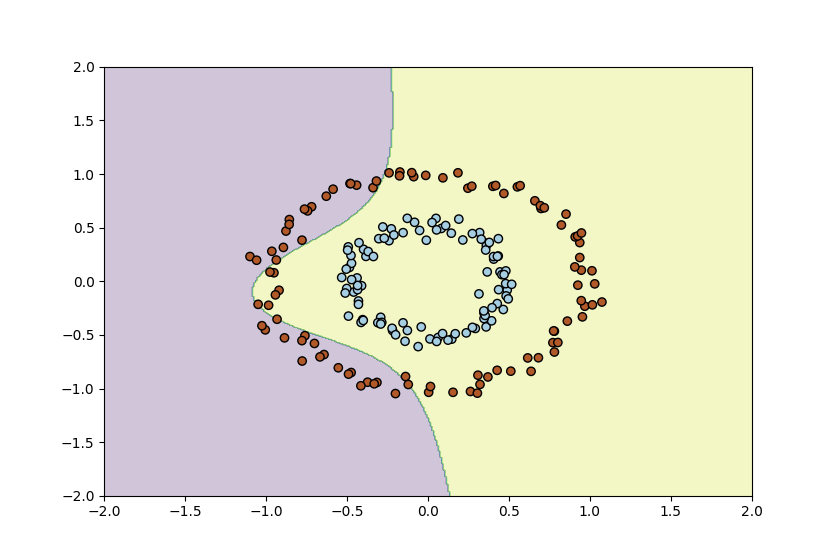
\includegraphics[scale=0.75]{svm-poly-2}
    \caption{Decision boundary of SVM with C = 2 and polynomial kernel}
\end{figure}
\begin{figure}
    \centering
    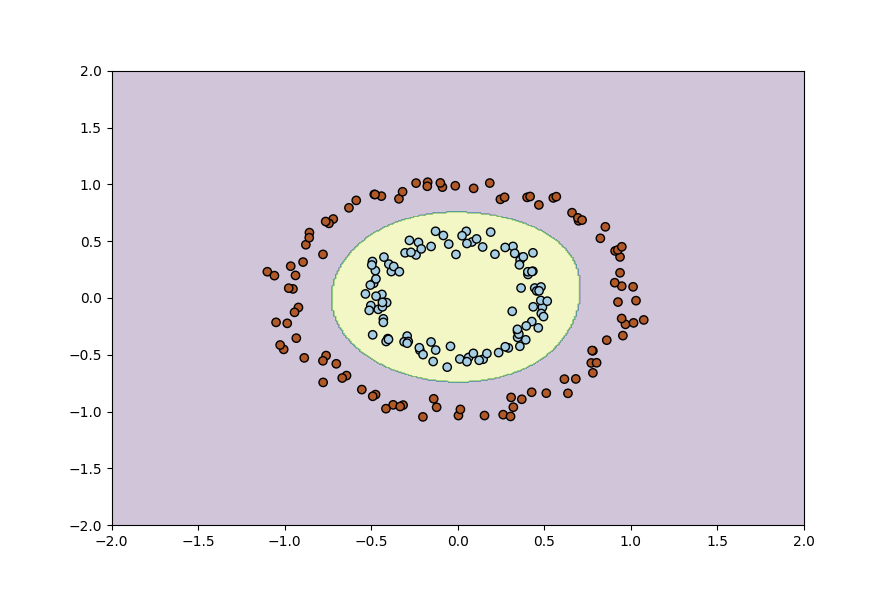
\includegraphics[scale=0.75]{svm-rbf-2}
    \caption{Decision boundary of SVM with C = 2 and rbf kernel}
\end{figure}


\section{Part 2}


\section{Part 3}





\end{document}